\documentclass[a4paper,12pt]{article}

\usepackage{latexsym}
\usepackage[utf8]{inputenc}
\usepackage{graphicx}

\author{Krzysztof~Palka and Dominik~Odrowski}

\title{\textsc{Exercise} 421 \\ Examination of light polarization by reflection phenomena} 

\addtolength{\textwidth}{2cm}
\addtolength{\hoffset}{-1cm}

\begin{document}

\maketitle

\begin{abstract}
    This report present the measurement of Brewster's angle for a given material. It shows relation of level of ray polarization depending on incident angle of unpolarized light.    
\end{abstract}
\section{Introduction}
    The aim of this exercise was determining of Brewster's angle for given material and, depending on obtained results, calculation of index of reflection. 


\section{Theory and measurement}
    The light polarized randomly (unpolarized) is characterized by electric filed at any given point perpendicular to the direction of travel of the waves but changes directions randomly. We can treat unpolarized light as combination of two perpendicular components (polarization S and P) which oscillate perpendicular to component of the electric field $\vec E$ (Fig. \ref{fig:sp}\footnote{\cite{HRW}, p. 901}).


\begin{figure}[ht]
    \begin{center}
        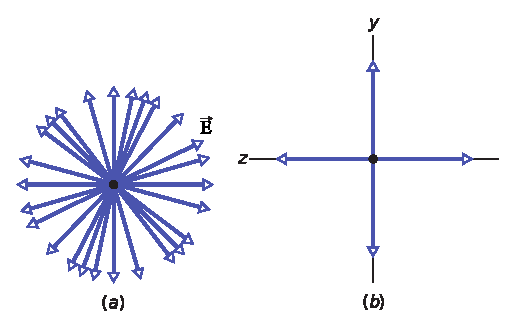
\includegraphics[width=0.60\textwidth]{simplified_polarization}
        \caption{polarization (a) could be simplified as (b).}
        \label{fig:sp}
    \end{center}
\end{figure}
\begin{figure}[ht]
\begin{center}
    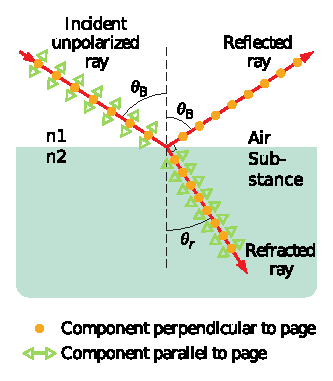
\includegraphics[width=0.35\textwidth]{brewster}
    \caption{direction of oscillations of incident, reflected and refracted rays.}
    \label{fig:brewang}
\end{center}
\end{figure}
Reflected ray is at least partially polarized. When ray incident on dielectric surface with angle $\theta_B$ (Fig. \ref{fig:brewang}\footnote{Ibid., p. 912}), that:
\begin{equation}
    \tan \theta_B = n \label{eq:brew_ang}
\end{equation}
where $n$ is the index of reflection of dielectric, then $\theta_B$ is called Brewster's angle and reflected ray is linearly polarized (electric field vectors on Fig. \ref{fig:brewang} oscillate perpendicular to the page). Incident rays oscillate in perpendicular and parallel directions, so they are unpolarized. Reflected ray behave in similar way, but magnitudes of particular components of electric field oscillations are unequal and that ray is called partially polarized. If incident angle is not equal Brewster's angle, then Reflected ray is also called partially polarized, and level of polarization $K$ can be obtained form equation \ref{eq:K}
\begin{equation}
    K = \frac{I_S-I_P}{I_S+I_P} \label{eq:K}
\end{equation}
Where $I_S$ and $I_S$ are intensities of lights with polarization S and P, according to figure \ref{fig:brewang} respectively perpendicular and parallel to plane determined by diagram.

\begin{figure}[ht]
\begin{center}
    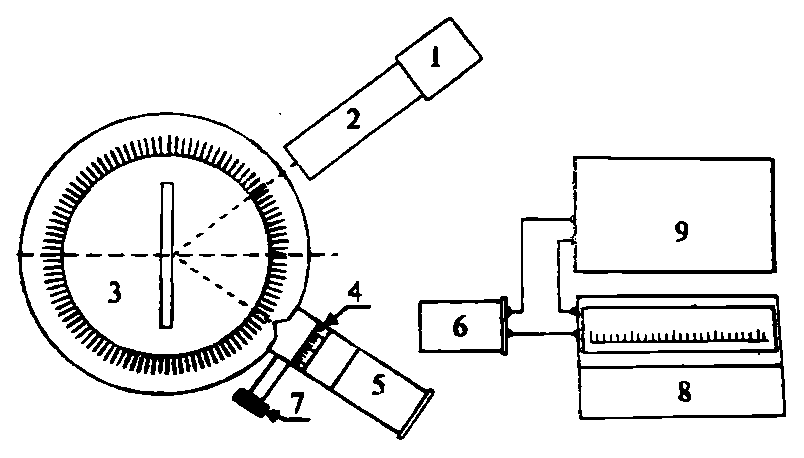
\includegraphics[width=0.85\textwidth]{goniometer}
    \caption{Diagram of the experimental set-up. It consists of swivel table (3) with angular scale of precision $\Delta\alpha = \pm 1^\circ$ and 2 arms. illumination (1) with collimator (2) is placed on fixed arm, analyser (4) and telescope on which could be placed eyepiece (5) or photodetector (6) are mounted on movable arm. Electric circuit consists of photoresistor which is used as photodetector (6), power supply unit (9) and microamperemeter (8).}
    \label{fig:goniometer}
\end{center}
\end{figure}

\begin{table}[t]
    \begin{center}
    \caption{Measured results: quantities $I_S$ and $i_P$ read form mikroamperometer for setted angle $\alpha$ and level of polarization calculated form equation \ref{eq:K}}
    \label{tab:results}
    \begin{tabular}{|c|c|c|c|}
          \hline
          $\alpha [^{ \circ }]$  & \
          $i$_S [$\micro$ A] \
          & $i$_P[\micro A] \
          & $K$  \\ \hline 
          20 & 19.0 & 10.9 & 0.271 \\
          30 & 26.0 & 7.5 & 0.552 \\
          40 & 31.2 & 3.0 & 0.825 \\
          50 & 49.0 & 0.6 & 0.976 \\
          52 & 63.7 & 0.5 & 0.984 \\
          54 & 59.4 & 0.5 & 0.983 \\
          55 & 63.8 & 0.4 & 0.988 \\
          56 & 74.6 & 0.4 & 0.989 \\
          57 & 69.9 & 0.5 & 0.986 \\
          58 & 88.0 & 0.5 & 0.989 \\
          60 & 96.2 & 0.7 & 0.986 \\
          70 & 161.2 & 14.8 & 0.832 \\
          80 & 209.1 & 69.1 & 0.503 \\
          \hline
     \end{tabular}
 \end{center}
 \end{table}

\section{Results}

\begin{figure}[ht]
    \begin{center}
        \includegraphics[width=0.80\textwidth]{is}
        \caption{graph of current of polarization S versus angle of incident, with measurement uncertainty of microamperometer $\pm(1.5\% + 1)$ for resolution 0.1}
        \label{fig:is}
    \end{center}
\end{figure}

\begin{figure}[ht]
    \begin{center}
        \includegraphics[width=0.80\textwidth]{ip}
        \caption{graph of current of polarization P versus angle of incident, with measurement uncertainty of microamperometer $\pm(1.5\% + 1)$ for resolution 0.1}
        \label{fig:ip}
    \end{center}
\end{figure}


\begin{figure}[ht]
    \begin{center}
        \includegraphics[width=0.80\textwidth]{pollev}
        \caption{Calculated level of polarization $K$ versus angle of incident.}
        \label{fig:pollev}
    \end{center}
\end{figure}

The results of our measurement are presented in Table \ref{tab:results}. It contains values of current flowing through photoresistor of light with polarization S and P for a given angle read from microamperemeter. It contains also level of polarization for a given angle calculated from equation \ref{eq:K}. Figures \ref{fig:is} and \ref{fig:ip} presents obtained values on a graph. Uncertainty of horizontal axis is $\pm 1^{\circ}$ because of scale of goniometer. Figure \ref{fig:pollev} presents level of polarization calculated from equation \ref{eq:K} and measurement uncertainty calculated  form equation \ref{eq:Ku} where $\Delta i$ is measurement uncertainty of current flowing through photodetector. Maximum level of polarization was noticed at the angle $56^{\circ}$, so according to equation \ref{eq:brew_ang} index of reflection of examined material is $n = \tan 56^{\circ} \approx 1.48 $. Because the light is not monochromatic, this is average index of refraction. After consideration of equation \ref{eq:Ku}, the level of polarization for angle $56^{\circ}$ would looks like $K = 0.989\pm 0.004$. To obtain uncertainty of index of reflection we use formula \ref{eq:nu}. So overall result of measuring index on reflection would look like.
\begin{equation}
    n = 1.48 \pm \Delta n = 1.48 \pm \frac{2\cdot 1.48}{\sin (2 \cdot 56^{\circ})} 0.0349 = 1.48 \pm 0.11 \label{eq:nuv}
\end{equation}


\begin{equation}
    \Delta K = \frac{2\Delta i}{i_S+i_P} \label{eq:Ku}
\end{equation}

\begin{equation}
    \Delta n = \frac{2n}{\sin 2 \alpha_B} \Delta \alpha_B \label{eq:nu}\end{equation}

\section{Conclusions} 
Even small change of values obtained form microamperometer leads to setting of wrong Brewster's angle. In conditions of measurement where there is not dark, mikroamperometer's indication could be easily disturbed, and as it is shown on fig. \ref{fig:pollev} values of $K$ in range $50^{\circ} - 60^{\circ}$ are very similar, so we could read not exactly Brewster's angle, but angle with similar polarization.

\begin{thebibliography}{9}
    \bibitem[HRW]{HRW}Fundamentals of physics (2011) [ebook]. David Halliday, Robert Resnick, Jearl Walker. 9th ed. ISBN 978-0-470-46908-8
\end{thebibliography}

\end{document}

